\documentclass[12pt]{article}

\usepackage{fancyhdr}
\usepackage{amsthm}
\usepackage{amsmath}
\usepackage{graphicx}
\usepackage{amssymb}
\usepackage{esint}
\usepackage{subfigure}
\usepackage{color}
\usepackage{moreverb}
\usepackage{wrapfig}

\textwidth 17cm \topmargin -1cm \oddsidemargin 0cm \textheight 21.5cm
\pagestyle{empty} \pagestyle{fancyplain}
\lhead[\fancyplain{}{}]{\fancyplain{}{{\sc Adam Farnsworth, Myles Adams:}}}
\chead[\fancyplain{}{}]{\fancyplain{}{{\sc Hw 2}}}
\rhead[\fancyplain{}{}]{\fancyplain{}{{\sc Fall 2017}}}

\newcommand{\etal}{\textit{et al. }}

\begin{document}
\centerline{\Large\textbf{Homework 2}}
\vspace{2cm}

\section{Introduction}\label{sec::Intro}
The goal of this project is to simulate the motion of a ball bouncing off the walls of a closed container.  When the ball interacts with the walls, friction forces are applied and the respective velocities are dampened.  The motion of the ball is described by the
system of second-order differential equations:
 \begin{eqnarray}
\frac{d^2x}{dt^2} &= &0 \\\nonumber
\frac{d^2y}{dt^2} &= &-g\\\nonumber
       \end{eqnarray}
with initial conditions:
 \begin{eqnarray}
x(0) = x^0, \frac{dx}{dt}(0) &= &v^0_x \\\nonumber
y(0) = y^0, \frac{dx}{dt}(0) &= &v^0_y \\\nonumber
       \end{eqnarray}
The position of the ball starts with: x and y coordinates $ (0.1, 0.7)$ in meters, initial velocities $(3,1)$ in  $\frac{m}{s}$ , damping coefficients $\alpha = 0.8, \beta = 0.9$, and gravity $g = 9.81 \frac{m}{s^2}$.


\section{Solving the problem}\label{sec::Solving the problem}
We can take the original equations that we have a represent them as a system of equations for both the x and y directions. We do this by splitting the equations up into position and velocity for each of the directions. The velocity in the x direction does not change unless it impacts any of the walls, this is due to newton's 1st law.  The velocity in the y direction is constantly affected by acceleration from gravity, and the impacts when colliding with any of the walls as well.  The equation for position in the y direction is modeled using the trapezoidal method as follows:
\begin{eqnarray}
y_{n+1} = y_{n} + \frac{1}{2} dt (Vy_{n}+Vy_{n+1})\nonumber
\end{eqnarray}
Velocity in the y direction for: free falling, right wall collision, left wall collision, bottom wall collision, and top all collision is modeled by:
\begin{eqnarray}
Vy_{n+1} &=& Vy_{n} - (g)(dt)  \\\nonumber
Vy_{n+1} &=& \beta(Vy_{n} - (g)(dt)) \\\nonumber
Vy_{n+1} &=& \beta(Vy_{n} - (g)(dt))  \\\nonumber
Vy_{n+1} &=& - \alpha(Vy_{n} - (g)(dt)) \\\nonumber
Vy_{n+1} &=& - \alpha(Vy_{n} - (g)(dt)) \\\nonumber 
\end{eqnarray}
The equation for position in the x direction is modeled using the trapezoidal method as well. Although, the two velocities used are always identical because the velocity only changes when the ball impacts a wall. But we still model it as follows:
\begin{eqnarray}
x_{n+1} = x_{n} + \frac{1}{2} dt (Vx_{n}+Vx_{n+1})\nonumber
\end{eqnarray}
Velocity in the x direction for: free falling, right wall collision, left wall collision, bottom wall collision, and top all collision is modeled by:
\begin{eqnarray}
Vx_{n+1} &=& Vx_{n}  \\\nonumber
Vx_{n+1} &=& - \alpha(Vx_{n}) \\\nonumber
Vx_{n+1} &=& - \alpha(Vx_{n})  \\\nonumber
Vx_{n+1} &=& \beta(Vx_{n}) \\\nonumber
Vx_{n+1} &=& \beta(Vx_{n}) \\\nonumber 
\end{eqnarray}


\section{Approach to model interactions between the ball and the walls}
To deal with the moment when the ball interacts with the wall, some instant of time $t_{n+1}$ the ball will be placed inside the wall.  We also need to take into account the radius of the ball, so more accurately  we will use $x_{n+1} +r > x_{wall}$.  To denote the time that the ball interacts with the wall $x = x_{wall} - r$ we will use the time $t^*_{n+1}$.  The intersection of a straight line with the side wall can be seen in the equation below:
\begin{eqnarray}
x_{wall} - r= x_{n} + \frac{x_{n+1}-x_n}{\Delta t} (t^*_{n+1}-t_n)\nonumber
\end{eqnarray}
we can then use this equation to get $t^*_{n+1}$ by putting it in the form:
\begin{eqnarray}
t^*_{n+1} = t_n + \Delta t \frac{x_{wall}-x_n - r}{x_{n+1} - x_n} \nonumber
\end{eqnarray}
Now that we have the time that the ball interacts with the wall, it can be used to calculate the reduced time step for the new time the ball is placed right next to the wall.


\section{Results obtained}
The following tables show the max error and order of accuracy using Trapezoidal at time $t = 0.931$ for the time steps $\Delta t = 0.02s, 0.01s, 0.005s, 0.0025s, 0.00125s, 0.000625s$ for x, y position and velocity in the x,y direction




\begin{table}[bht]
\begin{center}
\begin{tabular}{|l|c|r|c|c|}
\hline
Time-Step& Max Error & Order \\ \hline
0.02&$2.24134\cdot10^{-5}$& 1.90241\\ \hline
0.01& $5.99548\cdot10^{-6}$& 2.19067 \\ \hline
0.005& $1.31331\cdot10^{-6}$& 1.71910\\ \hline
0.0025& $3.98901\cdot10^{-7}$& 3.10524 \\ \hline
0.00125&$4.63547\cdot10^{-8}$& 1.23618 \\ \hline
0.000625& $1.96774\cdot10^{-8}$& 1.63811 \\ \hline

\end{tabular}
\quad
\begin{tabular}{|l|c|r|c|c|}
\hline
Time-Step& Max Error & Order \\ \hline
0.02& 0.000514115& 1.90277 \\ \hline
0.01& 0.000137489& 2.19077 \\ \hline
0.005& $3.01147\cdot10^{-5}$& 1.71912 \\ \hline
0.0025&$9.14684\cdot10^{-6}$& 3.10525 \\ \hline
0.00125& $1.06291\cdot10^{-6}$& 1.23617 \\ \hline
0.000625& $4.51202\cdot10^{-7}$& 1.63812 \\ \hline

\end{tabular}
\caption{x and y position}
\end{center}
\end{table}



\begin{table}[bht]
\begin{center}
\begin{tabular}{|l|c|r|c|c|}
\hline
Time-Step& Max Error & Order \\ \hline
0.02& 0.000000&  \\ \hline
0.01& 0.000000&  \\ \hline
0.005& 0.000000&  \\ \hline
0.0025& 0.000000&  \\ \hline
0.00125& 0.000000&  \\ \hline
0.000625& 0.000000&  \\ \hline

\end{tabular}
\quad
\begin{tabular}{|l|c|r|c|c|}
\hline
Time-Step& Max Error & Order \\ \hline
0.02& 0.001842& 1.90242 \\ \hline
0.01& 0.000492853& 2.19067 \\ \hline
0.005& 0.000107959&  1.71909\\ \hline
0.0025& $3.27914\cdot10^{-5}$& 3.10525 \\ \hline
0.00125& $3.81055\cdot10^{-6}$& 1.23618 \\ \hline
0.000625&$1.61756\cdot10^{-6}$& 1.63812 \\ \hline

\end{tabular}
\caption{x and y velocity}
\end{center}
\end{table}


\begin{figure}[h]
\begin{center}
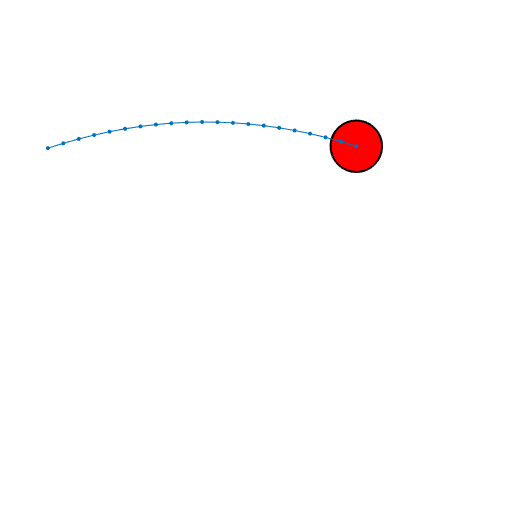
\includegraphics[width=.3\textwidth]{02}
\end{center}
\caption{Simulation at time t = 0.2, for $\Delta t = 0.01$} \label{fig::MyFigure}
\end{figure}

\begin{figure}[h]
\begin{center}
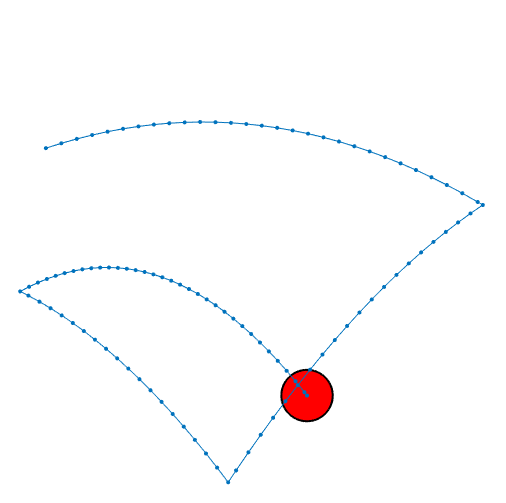
\includegraphics[width=.3\textwidth]{1}
\end{center}
\caption{Simulation at time t = 1, for $\Delta t = 0.01$} \label{fig::MyFigure}
\end{figure}

\begin{figure}[h]
\begin{center}
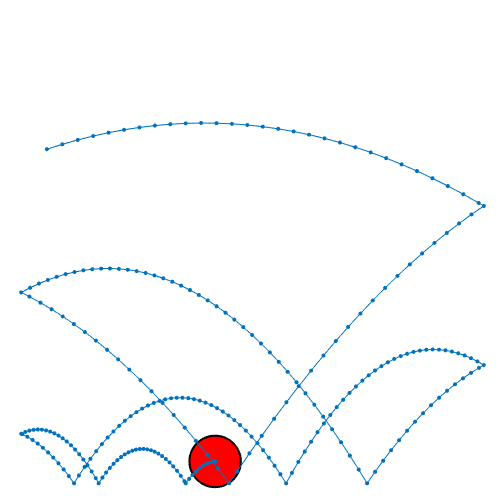
\includegraphics[width=.3\textwidth]{25}
\end{center}
\caption{Simulation at time t = 2.5, for $\Delta t = 0.01$} \label{fig::MyFigure}
\end{figure}








%%%%%%%%%%%
\newpage
\clearpage
\setcounter{page}{1} \pagestyle{empty}
\section{References}\label{sec::References}
\begin{itemize}
\item [1] Daniil Bochkov, CS 111 - Introduction to Computational Science Homework 2 Fall 2017
\item [2] Daniil Bochkov, CS 111 - Introduction to Computational Science Lecture 7 High-Order ODEs 2017

\end{itemize}


%%%%%%%%%%%

\end{document}
